\documentclass[serif,envcountsect,table,t,handout]{beamer}%, handout
\usepackage{amsmath, animate, hyperref, subcaption, tikz, multirow}
\usepackage{listings}
\usetheme{CambridgeUS}
\usecolortheme{wolverine}
% \usecolortheme{orchid}
\setbeamertemplate{navigation symbols}{}
\graphicspath{{../figures/}}
\addtobeamertemplate{frametitle}{}{\vspace{-3mm}} % reduce top space
%%%%----------------------------------------------------------
\begin{document}
\title[Estimation]{Pre College Summer - Data Science\\
Estimation: A Hide-and-Seek Game with the Nature}
\author[Bar, Wang]{Haim Bar, HaiYing Wang}
\date[]{}
\institute[UConn]{\normalsize University of Connecticut}
%%%% -------------------------------------------------
\begin{frame}[noframenumbering] \titlepage \end{frame}
%%%% ----------------------------------------------------------
\begin{frame}{Estimation}
  \begin{enumerate}
  \item When data are collected from some population, it contains information
    about it.
\item Estimation is the process of
using the observed data to estimate the unknown target population
quantities.
\item This process is like a hide-and-seek game that we play with the
Mother Nature.
\item The true features of the data-generating process are unknown.
\item We
estimate them using clues contained in the observed data.
  \end{enumerate}
\end{frame}
%%%% ----------------------------------------------------------
\begin{frame}{A simple hide-and-seek game}
  \begin{enumerate}
  \item Suppose we are interested in the true mean of the hight of all the boys of age
    12 in the US.
  \item Suppose that we observe a random sample of $n$ boys.
\item Our goal is to estimate the unknown
 $\mu$ using what we see from the random sample.

  \end{enumerate}
\end{frame}
%%%% ----------------------------------------------------------
\begin{frame}{Quality of an estimator}
  \begin{enumerate}
  \item A good estimator may by chance behaves worse than a bad estimator for a specific sample.
\item This variation of the estimator across different samples is called the
  variance.
\item The average of the estimator over all possible samples is called the
  expectation.
\item The difference of this expectation from the target is called the bias.
\item If the bias is zero, the estimator is \emph{unbiased}.
  \end{enumerate}
\end{frame}
%%%% ----------------------------------------------------------
\begin{frame}{Bias vs Variance}
  \begin{center}
    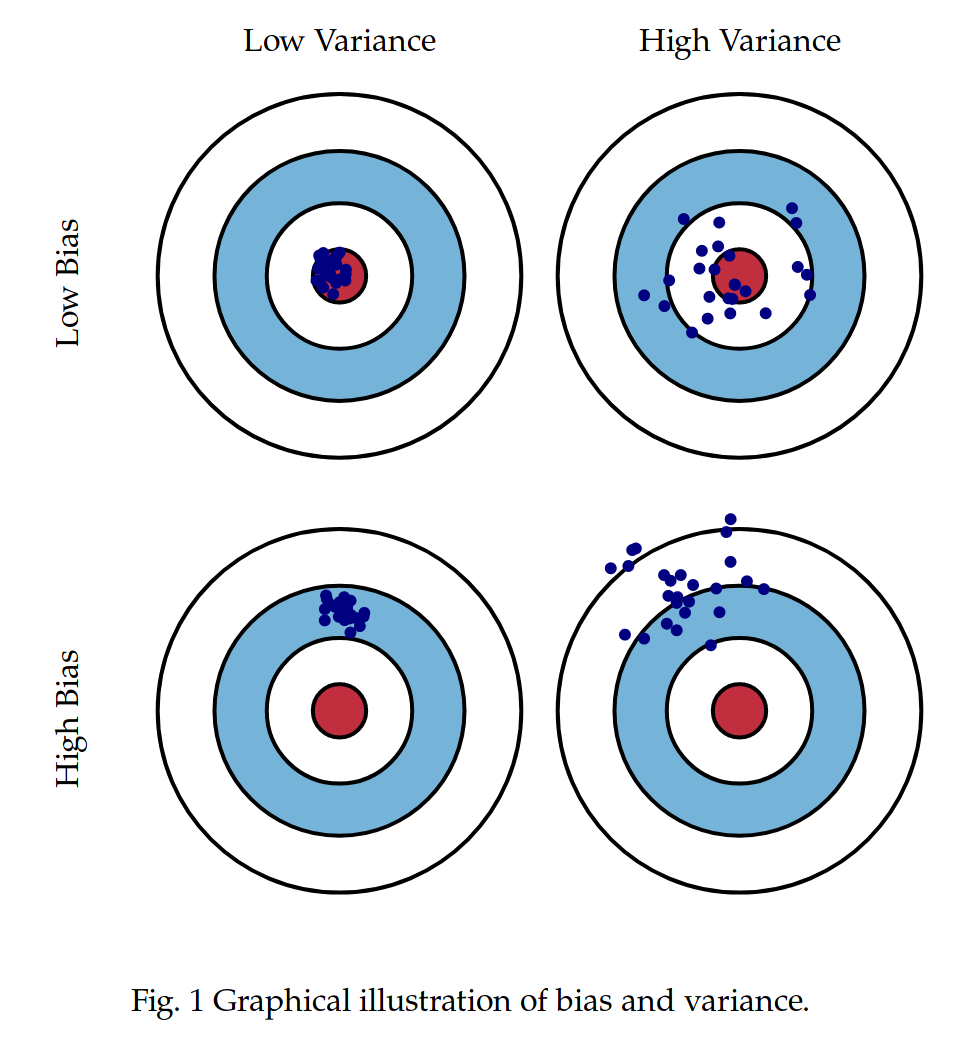
\includegraphics[width=0.7\textwidth]{biasvariance.png}
  \end{center}
\end{frame}
%%%% ----------------------------------------------------------
\begin{frame}{Mean squared error}
  \begin{enumerate}
\item The
expectation of the squared distance between an estimator and its target,
$E[(\hat\theta - \theta)^2]$, is the \emph{mean squared error (MSE)}.
\item The MSE is the sum of the variance and the square of the bias.
\item  An estimator with a smaller MSE than another estimator is
more \emph{efficient}.
  \end{enumerate}
\end{frame}
%%%% ----------------------------------------------------------
\begin{frame}{Non-normal populations}
  \begin{enumerate}
  \item What happens when the data is not normal?
  \item Now let us generate data from a distribution that has heavier tails than the
normal distribution.
\item For a heavier-tailed distribution, we are more likely to
observe extreme-valued observations.
\item We will also try uniform distribution.
% \item  Now it seems we can recycle
% the \lstinline{do1rep} function and make it more general by taking a data
% generation scheme as an input.
  \end{enumerate}
\end{frame}
%%%% ----------------------------------------------------------
\begin{frame}{Maximum Likelihood Estimator}
  Example: likelihood in guessing jars
  \begin{itemize}
\item There are 9 jars.
    \begin{enumerate}
    \item 9 red and 1 green balls;
    \item 8 red and 2 green balls;
    \item $\cdots\cdots$;\setcounter{enumi}{8}
    \item 1 red and 9 green balls.
    \end{enumerate}
  \item Now, one ball is randomly selected from one of the jars. 
  \item If the ball is red, which jar will you guess as the one that was selected?

% The first one!

\end{itemize}
\end{frame}
%%%% ----------------------------------------------------------
\begin{frame}{Maximum likelihood estimation}
  \begin{enumerate}
  \item The principle that we use here is the so-called \emph{maximum likelihood
estimation}\index{maximum likelihood estimation}.
\item The \emph{parameter
space}\index{parameter space}, that is, the collection of all possible values of
the parameter, consists of only 9 jars. 
\item We choose the one that gives the highest
likelihood of observing a randomly selected ball being red.

\item 
For problems with continuous parameter spaces, the principle remains the
same.
% \item In R, a convenient function for finding MLE for univariate
% distributions is \lstinline{fitdistr} in package \lstinline{MASS}.
  \end{enumerate}
\end{frame}
%%%% ----------------------------------------------------------
\begin{frame}{A simple example: Coin tosses}
  \begin{enumerate}
  \item Suppose we have a coin that we suspect is biased.
  \item Let the probability of getting a Head be $p$ and the probability of
  getting a Tail be $1-p$.
\item How do we find that value of $p$?
\item Let's toss the coin five times. Assume we get: H,T,T,H,H.
\item The probability of seeing this result is
  \begin{equation}
    L(p) = p(1-p)(1-p)p^2 = p^3(1-p)^2
    \label{eq:1}
  \end{equation}
\item Here $L(p)$ is the likelihood function.
\item The MLE of $p$ is the value of $p$ that maximizes $L(p)$.
\item It is often easier to maximize the log-likelihood function.
  \begin{equation}
    \ell(p) = \log L(p) = 3\log p + 2 \log(1-p). 
    \label{eq:2}
  \end{equation}
\end{enumerate}
\end{frame}
%%%% ----------------------------------------------------------
\begin{frame}{A point estimate may be as bad as a made up number}
  \begin{center}
    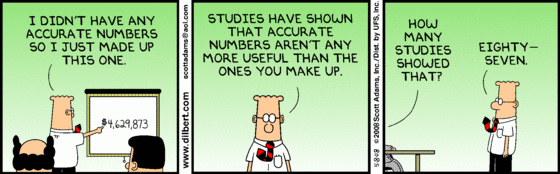
\includegraphics[width=\textwidth]{madeup.png}
  \end{center}
\end{frame}
%%%% ----------------------------------------------------------
% \begin{frame}{Uncertainty}
\begin{frame}{Interval estimation}
  \begin{enumerate}
  \item Point estimation is not enough!
  \item We need some measure of uncertainty to make
inferences.
\item This lead to interval estimators.
\item The two endpoints of an interval
estimator are statistics such that the random interval formed by them captures
the unknown target parameter with certaiin probability.
\item A \emph{confidence interval}\index{confidence interval} with
\emph{confidence level}\index{confidence level} $1-\alpha$ means an interval
estimator of the target parameter such that the probability that the interval
covers the target is~$1-\alpha$.
  \end{enumerate}
\end{frame}
%%%% ----------------------------------------------------------
\begin{frame}{}
  \begin{enumerate}
  \item The CLT tells us that the sample mean $\bar X_n$ is approximately
    \begin{equation}
       N(\mu, \sigma^2 / n).
      \label{eq:3}
    \end{equation}
    \begin{center}\-\\[-12mm]
      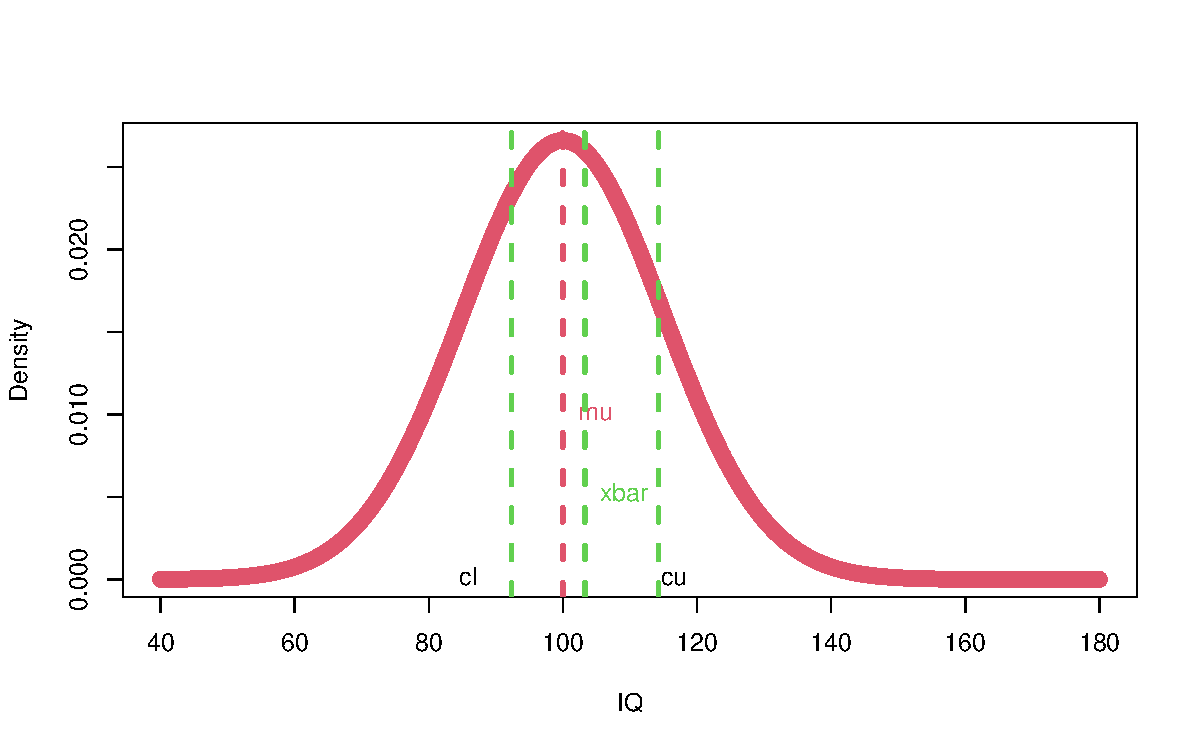
\includegraphics[width=0.8\textwidth]{ciIQ.pdf}\-\\[-12mm]
    \end{center}
\item We can construct a confidence interval for $\mu$ as $(cl, cu)$, where
  \begin{align}
    cl&=\bar X_n - z_{\alpha/2} \sigma/\sqrt{n}\\
    cu&=\bar X_n + z_{\alpha/2} \sigma/\sqrt{n})
\end{align}
  \end{enumerate}
\end{frame}
%%%% ----------------------------------------------------------
\begin{frame}{A CI may not always cover the true parameter}
    \begin{center}
      
\includegraphics[width=\textwidth]{ci.pdf}
    \end{center}
\end{frame}
%%%% ----------------------------------------------------------
\begin{frame}{Resampling}
  \begin{enumerate}
  \item The variation of a point estimator, however, can be much more
difficult to obtain.
\item 
\emph{Bootstrap}\index{bootstrap}
is a powerful tool to approximate the uncertainty of an estimator.
\item A self-assisted approach, it approximates the variation of the sample by
treating the sample as a population and resample repeatedly from it with
replacement, each time forming a so-called bootstrap sample of the same size as
the original sample.
\item For each bootstrap sample, we can obtain the point
estimator.
\item The variation of the original point estimator can be approximated by
the empirical variation of a collection of the point estimators obtained from
the bootstrap samples.
  \end{enumerate}
\end{frame}
%%%% ----------------------------------------------------------
\begin{frame}{Example: estimate the median}
    \begin{center}
      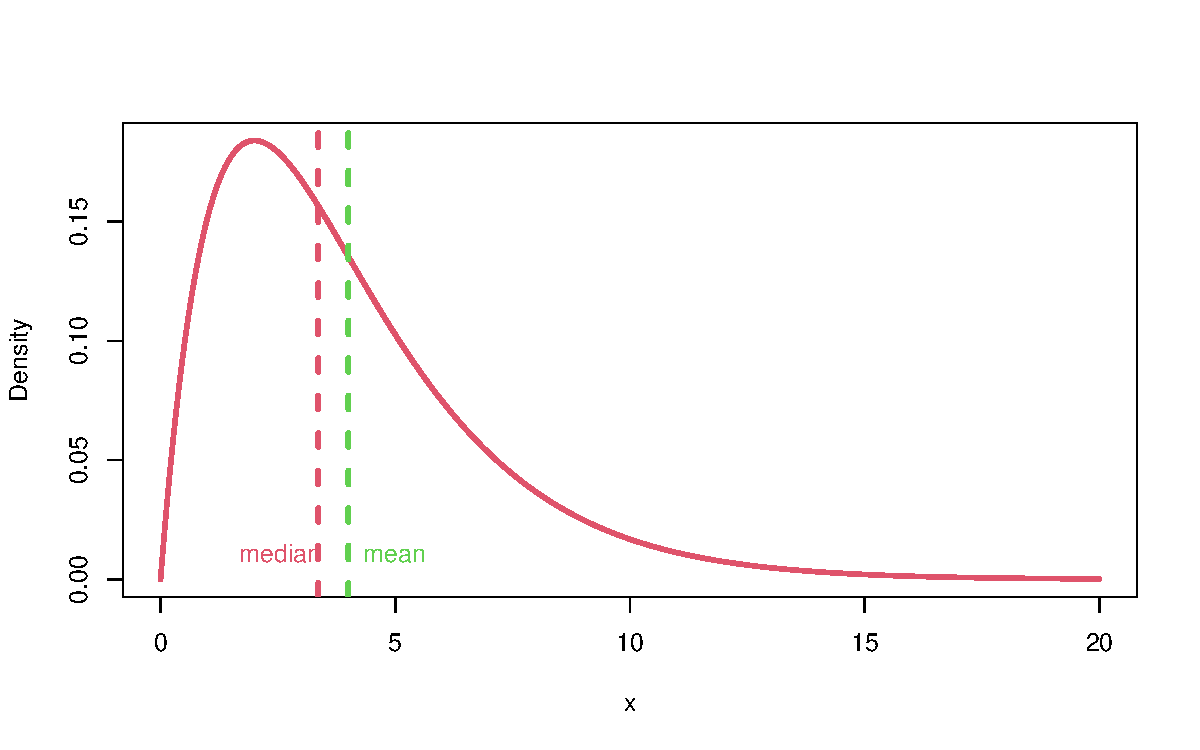
\includegraphics[width=\textwidth]{gammaMedian.pdf}
    \end{center}
\end{frame}
%%%% ----------------------------------------------------------
\end{document}

